\documentclass{IMTexam}

\usepackage{IMTtikz}
\DeclareSIUnit{\atm}{atm}
\DeclareSIUnit{\calorie}{cal}
\usepackage{mhchem}

\usepackage{listings,xcolor}

\lstset{language=Mathematica}
\lstset{basicstyle={\sffamily\footnotesize},
  numbers=left,
  numberstyle=\tiny\color{gray},
  numbersep=5pt,
  breaklines=true,
  captionpos={t},
  frame={lines},
  rulecolor=\color{black},
  framerule=0.5pt,
  columns=flexible,
  tabsize=2
}


\givecredits
\author{Isabella B. \& Joel B. \& Jonathan B.}
%\USPN{}
\lecture{Química II}
\examname{Prova III}
\hwtype{Resolução}
\lcode{}
\date{12 de julho}

\begin{document}
    \maketitle

    \begin{questions}
        \question Considere que a decomposição térmica do \ce{N2O5} gasoso
        segue o seguinte mecanismo:

        \begin{align*}
            &\ce{N2O5}\overset{k_1}{\longrightarrow}\ce{NO2}+\ce{NO3}\\
            &\ce{NO2}+\ce{NO3}\overset{k_1}{\longrightarrow}\ce{N2O5}+\ce{NO3}\\
            &\ce{NO2}+\ce{NO3}\overset{k_2}{\longrightarrow}\ce{NO2}+\ce{O2}+\ce{NO}\\
            &\ce{NO}+\ce{N2O5}\overset{k_3}{\longrightarrow}\ce{3NO2}
        \end{align*}

        \begin{parts}
            \part Usando a aproximação do estado estacionário para as espécies
            \ce{NO3} e \ce{NO}, obtenha a lei cinética derivada do mecanismo
            proposto.

            \begin{solution}
                Aproximações de estado estacionário:
                \begin{equation}
                    \label{no3rate}
                    \dod{[\ce{NO3}]}{t} = 0 = k_{1}[\ce{N2O5}] - (k_{-1}[\ce{NO2}][\ce{NO3}] + k_{2}[\ce{NO2}][\ce{NO3}])
                \end{equation}

                \begin{equation}
                    \label{norate}
                    \dod{[\ce{NO}]}{t} = 0 = k_{2}[\ce{NO2}][\ce{NO3}] - k_{3}[\ce{NO}][\ce{N2O5}]
                \end{equation}

                Isolamos os intermediários por álgebra:

                \begin{align*}
                k_{1}[\ce{N2O5}] &= [\ce{NO3}](k_{-1}[\ce{NO2}] + k_{2}[\ce{NO2}])\\
                [\ce{NO3}] &= \dfrac{k_{1}[\ce{N2O5}]}{k_{-1}[\ce{NO2}] + k_{2}[\ce{NO2}]}\\
                k_{2}[\ce{NO2}][\ce{NO3}] &= k_{3}[\ce{NO}][\ce{N2O5}]\\
                [\ce{NO}] &= \dfrac{k_{2}[\ce{NO2}][\ce{NO3}]}{k_{3}[\ce{N2O5}]}
                \end{align*}

                O intermediário $[\ce{NO}]$ depende de $[\ce{NO3}]$. Removemos essa dependência:

                \[ [\ce{NO}] = \dfrac{k_2[\ce{NO2}]}{k_{3}[\ce{N2O5}]} \cdot \dfrac{k_{1}[\ce{N2O5}]}{k_{-1}[\ce{NO2}] + k_{2}[\ce{NO2}]} \]

                \begin{equation}
                    \label{noconc}
                    [\ce{NO}] = \dfrac{k_{1}k_{2}}{k_{3}(k_{-1} + k_{2})}
                \end{equation}

                Determinamos a expressão para a lei cinética do mecanismo completo e substituimos valores que conhecemos via (\ref{no3rate}) e (\ref{norate}):
                \[\dod{[\ce{N2O5}]}{t} = k_{-1}[\ce{NO2}][\ce{NO3}] - (k_{1}[\ce{N2O5}] + k_{3}[\ce{NO}][\ce{N2O5}])\]

                \[\dod{[\ce{N2O5}]}{t} = -2k_{3}[\ce{NO}][\ce{N2O5}]\]

                Substituindo o valor de $[\ce{NO}]$ achado em (\ref{noconc}),
                \[\dod{[\ce{N2O5}]}{t} = -2\dfrac{k_{1}k_{2}}{k_{-1}+k_{2}}[\ce{N2O5}]\]
            \end{solution}

            \part Obtenha a lei cinética admitindo as reações (1) e (-1) como
            um equilíbrio.

            \begin{solution}
                Aproximação de pré-equilíbrio:

                \begin{align*}
                    k_{1}[\ce{N2O5}] &= k_{-1}[\ce{NO2}][\ce{NO3}]\\
                    [\ce{NO2}][\ce{NO3}] &= \dfrac{k_{1}}{k_{-1}}[\ce{N2O5}]
                \end{align*}

                Separamos o mecanismo em duas partes:

                 \[ \ce{N2O5 <=>[k_{1}][k_{-1}] NO2 + NO3 ->[k_{2}] NO2 + O2 + NO}\]

                 \[ \ce{NO + N2O5 ->[k_{3}] 3NO2}\]

                A aproximação de pré-equilíbrio assume que $k_{2} \ll k_{1}$ e $k_{-1}$, mas não nos diz nada sobre $k_{3}$. Dado o resultado da (a), é razoável assumir que a segunda parte do mecanismo é relativamente rápida, i.e que $k_{3} > k_{2}$. Logo, a etapa limitante é a etapa 2.

                Analisamos, então, a lei cinética para $\ce{NO}$ para a etapa 2:
                \[\dod{[\ce{NO}]}{t} = k_{2}[\ce{NO2}][\ce{NO3}]\]

                Pela aproximação de pré-equilíbrio:
                \[\dod{[\ce{NO}]}{t} = \dfrac{k_{1}k_{2}}{k_{-1}}[\ce{N2O5}] \]

                Essa é a etapa limitante, então é a nossa lei cinética. Para obtê-la para $[\ce{N2O5}]$, basta ajustar a estequiometria:
                \[ \dod{[\ce{N2O5}]}{t} = -2\dfrac{k_{1}k_{2}}{k_{-1}}[\ce{N2O5}]\]
            \end{solution}

            \part Mostre que da lei cinética obtida em (a) pode-se, através de
            aproximações, chegar à mesma equação obtida em (b). Em que
            condições está justificada essa aproximação? Teste sua hipótese
            utilizando valores plausíveis para as constantes de velocidade.

            \begin{solution}
                Como já foi dito, a aproximação de pré-equilíbrio assume que
                $k_{2} \ll k_{1}$ e $k_{-1}$. Se assumirmos isso para a equação
                obtida em a), podemos aproximar $k_{-1} + k_{2} \approx
                k_{-1}$, obtendo uma equação idêntica à b). Essa aproximação é
                a condição para fazermos a aproximação de pré-equilíbrio: se as
                etapas de equilíbrio forem muito mais rápidas que a etapa 2,
                então elas conseguem reestabelecer o equilíbrio mais
                rapidamente que a etapa 2 consegue desestabilizá-lo,
                justificando a aproximação que a condição de equilíbrio sempre
                vale.

                Podemos checar se vale dando valores numéricos para as
                constantes. Referenciando o NIST Chemical Kinetics Database,
                obtivemos os valores $k_{1} = 5 \cdot 10^{-2}$, $k_{2} =
                3,64*10^{-16}$ e $k_{-1} = 1,66 \cdot 10^{-12}$ para $T =
                \SI{298}{\kelvin}$ e
                para as ordens esperadas (1ª, 2ª e 2ª, respectivamente). Para
                esses valores, a equação de (a) fica:

                \[ \dod{[\ce{N2O5}]}{t} = -2\dfrac{\num{5e-2} \cdot
                \num{3,64e-16}}{\num{1,66e-12}+\num{3,64e-16}}[\ce{N2O5}] =
                -\dfrac{\num{3,64e-17}}{\num{1,66e-12}+\num{3,64e-16}}[\ce{N2O5}] \]

                O denominador da constante vale $ \num{1,660364e-12} $, que é
                aproximadamente $ \num{1,66e-12}$. Fica claro, então, que a
                aproximação é válida para valores experimentais das constantes.
            \end{solution}

        \end{parts}

        \question As reações paralelas de substituição nucleofílica bimolecular
        (\ce{SN2}) e eliminação bimolecular de formaldeído (\ce{E_{CO}2})
        observadas entre o nitrato de metila (\ce{MeNO3}) e o íon hidróxido
        foram estudadas e são representadas com suas respectivas constantes de
        velocidade abaixo:

        \begin{gather*}
            \ce{MeNO3}+\ce{HO-}\rightarrow \ce{CH3OH}+\ce{NO3-},k_{\ce{SN2}}\\
            \ce{MeNO3}+\ce{HO-}\rightarrow \ce{H2O}+\ce{CH2O}+\ce{NO2-},k_{\ce{E_{CO}2}}
        \end{gather*}

        Esse estudo experimental foi conduzido a uma temperatura e pressão
        constantes e em excesso de nitrato de metila, fornecendo os dados
        cinéticos a seguir. As reações também foram modeladas do ponto de vista
        teórico, fornecendo valores de energia relativos dos “reagentes” e dos
        estados de transição, conforme apresentado no diagrama a seguir.

        \begin{center}
            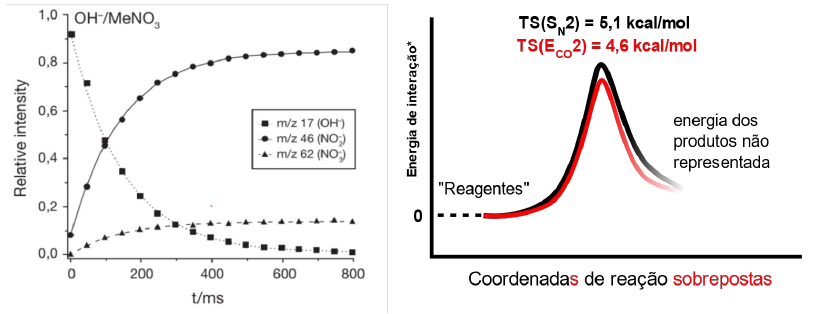
\includegraphics[width=\linewidth]{2021-08-01-12-33-20.png}
        \end{center}

        Os dados teóricos foram obtidos em um ótimo nível de cálculo e fornecem a
        estrutura dos reagentes e dos estados de transição abaixo, mesmo assim,
        sua precisão não é inferior a 1 kcal/mol.

        \begin{center}
            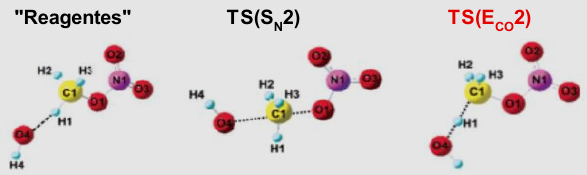
\includegraphics[width=\linewidth]{2021-08-01-12-33-35.png}
        \end{center}

        \begin{parts}
            \part Considerando que a intensidade relativa pode ser considerada
            como proporcional a concentração dos reagentes, escreva as
            derivadas $\od{[\ce{HO-}]}{t}, \od{[\ce{NO3-}]}{t},
            \od{[\ce{NO2-}]}{t}$ em função das constantes de velocidades e
            das concentrações das espécies envolvidas.

            \begin{solution}
                \begin{align*}
                    \dod{[\ce{OH-}]}{t}&=-k_{\ce{SN2}}[\ce{MeNO3}][\ce{OH-}]-k_{\ce{E_{CO}2}}[\ce{MeNO3}][\ce{OH-}]\\
                    &=\del{-k_{\ce{SN2}}-k_{\ce{E_{CO}2}}}[\ce{MeNO3}][\ce{OH-}]\\
                    &=-\del{k'_{\ce{SN2}}+k'_{\ce{E_{CO}2}}}[\ce{OH-}]
                \end{align*}

                Como temos um excesso de \ce{MeNO3}, segue que:
                \begin{gather*}
                    \dod{[\ce{NO3-}]}{t}=k_{\ce{SN2}}[\ce{MeNO3}][\ce{OH-}]=k'_{\ce{SN2}}[\ce{OH-}]\\
                    \dod{[\ce{NO2-}]}{t}=k_{\ce{E_{CO}2}}[\ce{MeNO3}][\ce{OH-}]=k'_{\ce{E_{CO}2}}[\ce{OH-}]
                \end{gather*}

                O que nos leva às relações:
                \begin{gather*}
                    \dod{[\ce{OH-}]}{t}=-k'_{\ce{SN2}}[\ce{OH-}]-k'_{\ce{E_{CO}2}}=-\del{k'_{\ce{SN2}}+k'_{\ce{E_{CO}2}}}[\ce{OH-}]\\
                    \dod{[\ce{NO3-}]}{t}=k'_{\ce{SN2}}[\ce{OH-}]\\
                    \dod{[\ce{NO2-}]}{t}=k'_{\ce{E_{CO}2}}[\ce{OH-}]
                \end{gather*}
            \end{solution}

            \part Com os dados cinéticos do gráfico (também apresentados na
            tabela no fim dessa questão), obtenha a constante de decaimento de
            \ce{HO-} experimental, os valores de $k_{\ce{SN2}}$ e $k_{\ce{E_{CO}2}}$.

            \begin{solution}
                Com
                \[ [\ce{OH-}]_{(t)}=[\ce{OH-}]_0\mathrm{e}^{-(k'_{\ce{SN2}}+k'_{\ce{E_{CO}2}})t} \]

                Podemos tomar
                \begin{align*}
                    \dod{[\ce{NO3-}]}{t}&=k'_{\ce{SN2}}\cdot[\ce{OH-}]_0\mathrm{e}^{-(k'_{\ce{SN2}}+k'_{\ce{E_{CO}2}})t}\\
                    \implies
                    \int_0^t \dif\,[\ce{NO3-}]&=k'_{\ce{SN2}}[\ce{OH-}]_0 \int_0^t \dif\mathrm{e}^{-\del{k'_{\ce{SN2}}+k'_{\ce{E_{CO}2}}}t}\dif t\\
                    \intertext{e, sendo $\int \mathrm{e}^{-x\,t}\dif t=-\mathrm{e}^{-x\,t}/x+C$, temos que}
                    [\ce{NO3-}]&=
                    k'_{\ce{SN2}}[\ce{OH-}]_0\cdot
                    \del{
                        -\dfrac{ \mathrm{e}^{ -\del{ k'_{\ce{SN2}} + k'_{\ce{E_{CO}2}} }t } }{ \del{ k'_{\ce{SN2}}+k'_{\ce{E_{CO}2}} } }
                        +
                        \dfrac{1}{ \del{ k'_{\ce{SN2}} + k'_{\ce{E_{CO}2}} } }
                    }\\
                    &= \dfrac{k'_{\ce{SN2}}[\ce{OH-}]_0}{k'_{\ce{SN2}}+k'_{\ce{E_{CO}2}}}\del{1-\mathrm{e}^{-\del{ k'_{\ce{SN2}} + k'_{\ce{E_{CO}2}} }t}}\\
                    \intertext{o que implica que $[\ce{NO2-}]\ce{->}\SI{100}{\percent}$ análogo e, portanto}
                    [\ce{NO2-}]&=\dfrac{k'_{\ce{SN2}}[\ce{OH-}]_0}{k'_{\ce{SN2}}+k'_{\ce{E_{CO}2}}}\del{1-\mathrm{e}^{-\del{ k'_{\ce{SN2}} + k'_{\ce{E_{CO}2}} }t}}
                \end{align*}

                Substituindo valores, temos:

                Para $\ce{OH-}$:
                \begin{align*}
                    \num{0.12}&=\num{0.93}\mathrm{e}^{-\del{k'_{\ce{SN2}} + k'_{\ce{E_{CO}2}}}300}\\
                    \implies \dfrac{12}{93}&=\mathrm{e}^{-\del{k'_{\ce{SN2}} + k'_{\ce{E_{CO}2}}}300}\\
                    \implies \log\del{\dfrac{12}{93}}&=-300\del{k'_{\ce{SN2}} + k'_{\ce{E_{CO}2}}}\\
                    \implies \del{k'_{\ce{SN2}} + k'_{\ce{E_{CO}2}}}&\approx \num{0.0068}\approx\num{6.8e-3}
                \end{align*}

                Para $\ce{NO3-}$:
                \begin{align*}
                    \num{0.12}&=k'_{\ce{SN2}}\cdot\num{0.93}\underbrace{\del{1-\underbrace{\mathrm{e}^{-\num{6.8e-3}\cdot300}}_{\num{0.13}}}}_{\num{0.87}}\\
                    \num{0.12}&=\dfrac{k'_{\ce{SN2}}\cdot\num{0.809}}{\num{6.8e-3}}
                \end{align*}
                o que nos dá
                \begin{align*}
                    \num{8.16e-4}&=k'_{\ce{SN2}}\cdot\num{0.809} & \num{6.8e-3}&=\num{1e-3}+k'_{\ce{E_{CO}2}}\\
                    k'_{\ce{SN2}}&\approx \num{1e-3} & k'_{\ce{E_{CO}2}}&\approx \num{5.8e-3}
                \end{align*}
            \end{solution}

            \part Mostre a partir das derivadas parciais que o valor da
            constante de decaimento de \ce{HO-} é igual a soma das outras
            constantes e mostre que isso se verifica com os valores calculados
            em b. A equação de Eyring relaciona o valor da constante de
            velocidade com a energia livre de ativação, que pode ser
            representada pela entalpia e entropia de ativação conforme a
            seguinte equação:

            \[ k(T)=\dfrac{k_bT}{h}\mathrm{e}^{\sfrac{\Delta S^{\ddagger}}{R}}\mathrm{e}^{-\sfrac{\Delta H^\ddagger}{RT}} \]

            \begin{solution}
                \begin{align*}
                    [\ce{OH-}]&=[\ce{OH-}]_0\mathrm{e}^{-k^*t}\\
                    \dod{[\ce{OH-}]}{t}&=\underbrace{[\ce{OH-}]_0\mathrm{e}^{-k^{*t}}}_{[\ce{OH-}]}\cdot\del{-k^*}=-k^*[\ce{OH-}]=-\del{k'_{\ce{SN2}}+k'_{\ce{E_{CO}2}}}[\ce{OH-}]
                \end{align*}
            \end{solution}

            \part Considerando que a energia de interação dos estados de
            transição é praticamente a mesma, explique porque a reação
            \ce{E_{CO}2} é mais rápida do que a \ce{SN2}.

            \begin{solution}
                Ao considerar que a energia de interação dos estados de
                transição é praticamente a mesma, a explicabilidade de a reação
                \ce{E_{CO}2} ser mais rápida do que \ce{SN2}, se deve ao fato
                de que a similaridade da estrutura eletrostática interna do
                componente não dificulta a velocidade de reação entre os
                componentes, isto é, devido à diferença de energia entre as
                estruturas internas dos elementos, com interações específica
                como as forças de interação de London, o que gera uma maior
                interação entre entre os elementos e diminui as velocidades de
                reação entre as moléculas.
            \end{solution}

            \part Com esses dados, é possível afirmar alguma coisa a respeito
            do papel do nitrato de metila no mecanismo da reação?

            Dados cinéticos:

            \begin{center}
                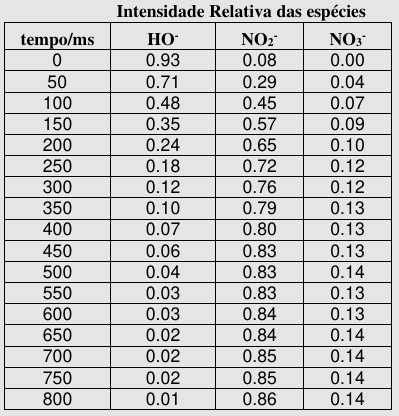
\includegraphics[width=0.5\linewidth]{2021-08-01-12-33-46.png}
            \end{center}

            \begin{solution}
                O incremento de nitrato de metila no mecanismo da reação
                estabiliza o equilíbrio da intensidade relativa das espécies
                químicas na reação, agindo como uma espécie de solução tampão,
                em que a intensidade relativa das espécies entre
                \SI{200}{\milli\second} até \SI{800}{\milli\second} se mantém
                em uma zona de estabilidade.
            \end{solution}
        \end{parts}

    \end{questions}
\end{document}
